\paragraph{Vertical Displacement $\delta$.}

When an obstacle hexagon is rotated by $\alpha_i$, the height of the obstacle hexagon becomes $h \sec \alpha_i$ where $h$ is the canonical height of the obstacle hexagon (see Figure \ref{fig:hexagonNonCanonical.pdf} for reference).
Figure \ref{fig:hexagonNonCanonical.pdf} shows the geometry of a rotated obstacle hexagon.

\begin{minipage}{\linewidth}
\begin{center}
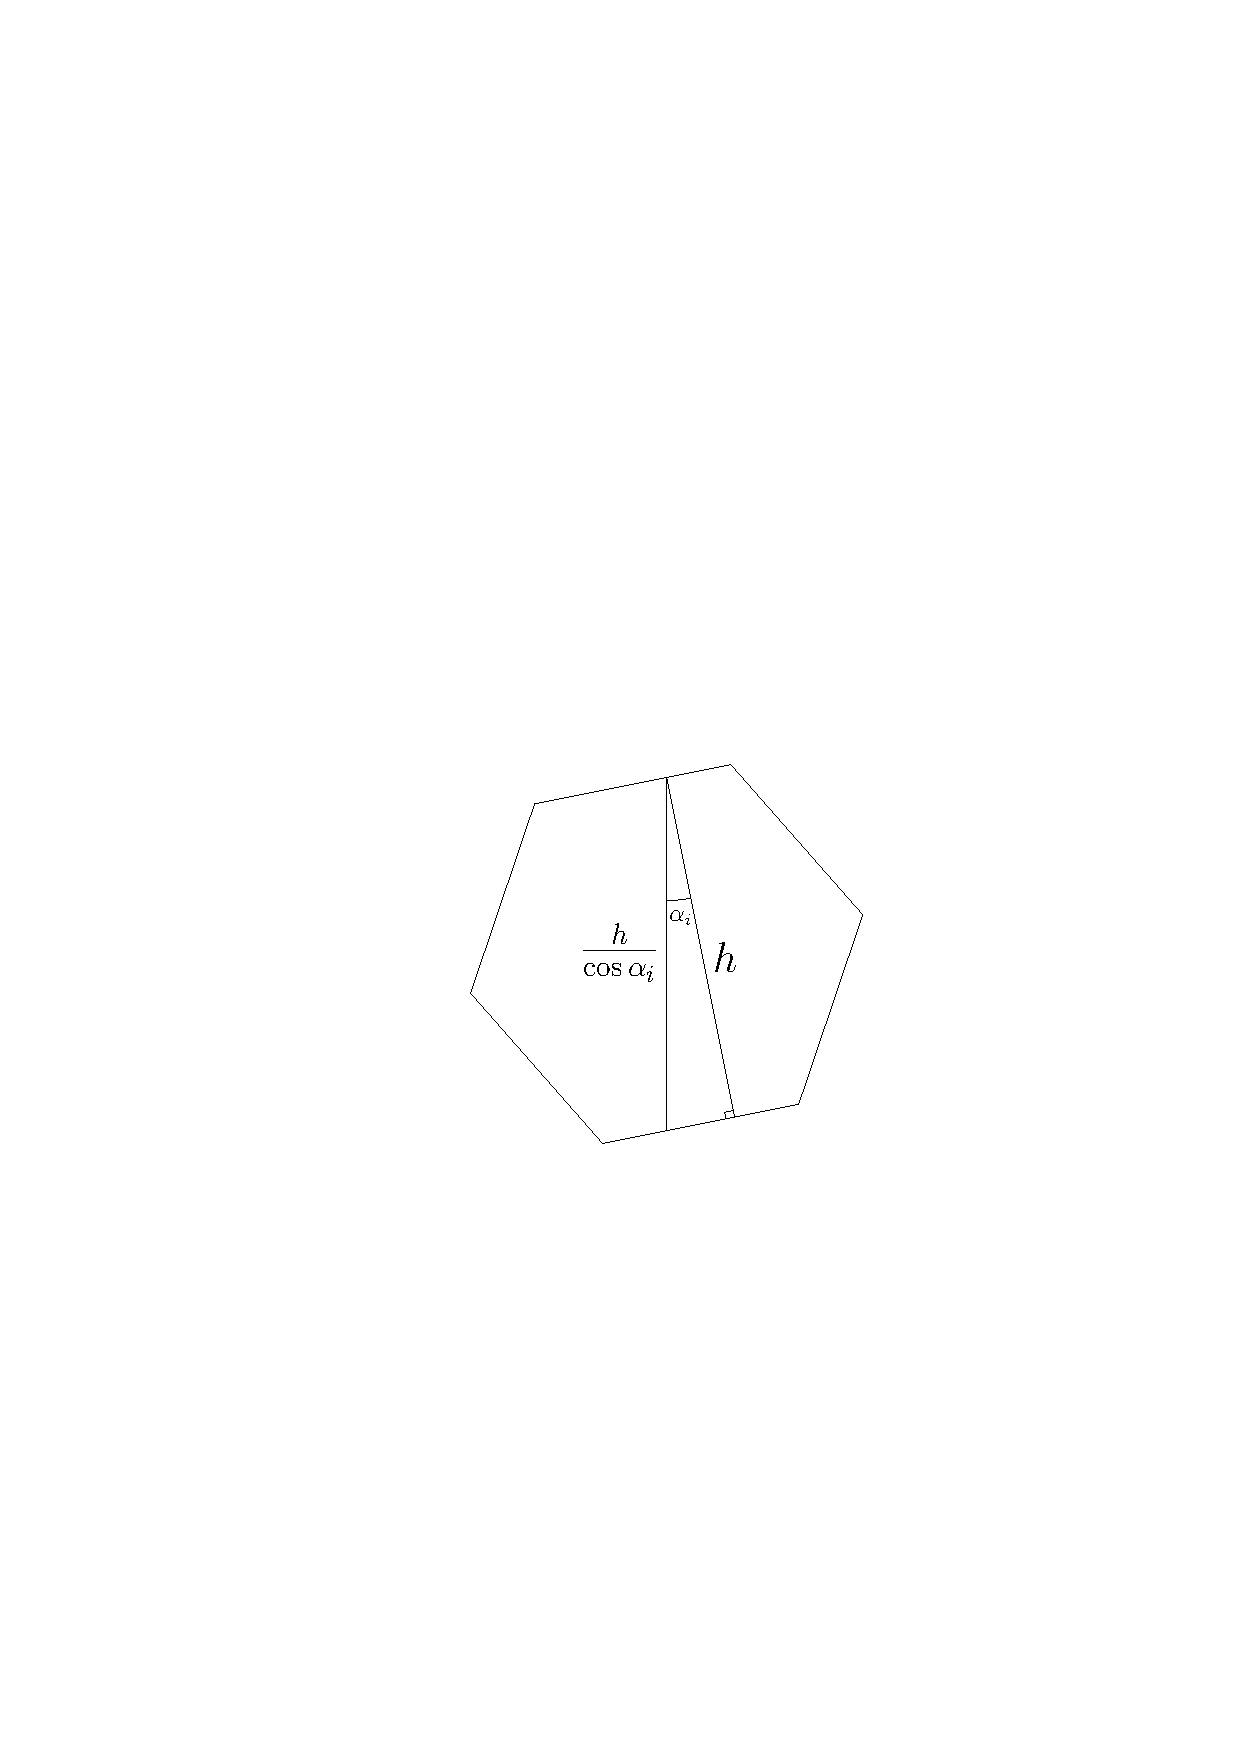
\includegraphics[width=.33\columnwidth]{graphics/hexagonNonCanonical2.pdf}
\captionof{figure}{
This figure shows a right triangle with angle $\alpha_i$ and sides of length $h$ and $\frac{h}{\cos \alpha_i}$.
}\label{fig:hexagonNonCanonical.pdf}
\end{center}
\end{minipage}

To show that the vertical displacement from canonical position is small, we first consider a column of obstacle hexagons in canonical position (see Figure \ref{fig:dualSmallHexagonalGrid.pdf} for illustration).  
For canonical position, the $\jth$ obstacle has $\delta_j = 0$.

\begin{minipage}{\linewidth}
\begin{center}
\includegraphics[width=.33\columnwidth]{graphics/verticalDisplacementArgument.pdf}
\captionof{figure}{This illustration is of a column of obstacle hexagons in canonical position along a vertical line segment $\ell$.}\label{fig:verticalDisplacementArgument.pdf}
\end{center}
\end{minipage}

From Equation \ref{eqn:Hnm}, we know the exact height of $\ell$ in terms of the heights of the corridors and obstacle hexagons in canonical position.
In Figure \ref{fig:verticalDisplacementArgument.pdf}, line segment $\ell$ is a vertical line segment passing through  the midpoint hinge of the lowestobstacle hexagon  because the rotational displacement is sufficiently small such that $\ell$ instersects \textit{all} obstacle hexagons in a column.  
Consider the entire column of obstacle hexagons and corridors for an arbitrary construction with angular rotation and vertical displacement for \textit{one} obstacle hexagon $\vert \delta_v \vert > 0$, where $j=2$, $\cdots$, $u+1$ and $1 < v \leq u+1$.
% Consider the first $j$ terms for the height of the column of obstacle hexagons and corridors for an arbitrary construction with angular rotation and vertical displacement for \textit{one} obstacle hexagon $\vert \delta_v \vert > 0$, where $j=2$, $\cdots$, $u+1$ and $1 < v \leq j$.
\begin{eqnarray*}
\sum_{i=1}^{u+1} \left[ \lr{2 \sqrt{3} N \sec \lr{ \alpha_i}} + \vlr{\delta_i - \delta_{i+1}} \right] + u \lr{\frac{1}{100N}+\sqrt{3}} &\leq& (u+1) 2 N \sqrt{3} + u  \lr{\frac{1}{100N}+\sqrt{3}}\\
2 \sqrt{3} N \sum_{i=1}^{u+1} \sec \lr{ \alpha_i} + \sum_{i=1}^{u+1} \vlr{\delta_i - \delta_{i+1}} &\leq& (u+1) 2 \sqrt{3} N \\
\vlr{\delta_i - \delta_{i+1}}\leq \sum_{i=1}^{u+1}\vlr{\delta_i - \delta_{i+1}} &\leq&  2 \sqrt{3} N \lr{(u+1) - \sum_{i=1}^{u+1} \sec \lr{ \alpha_i}}\\
&\leq& 2 \sqrt{3} N \sum_{i=1}^{u+1} \frac{\alpha_i^2}{2}\\
&\leq&  \sqrt{3} \frac{5s^\kappa - 1}{2} \lr{\frac{288}{s^{2-\kappa}}}^2 (u+1)\\ 
&\leq& \frac{6 \cdot 288^2 \cdot 13}{s^{-4+2\kappa + \lr{\kappa + 1}}}\\
&\leq&\frac{6469632}{s^{\kappa-3}}
\end{eqnarray*}
For when $1< j\leq u$, we have the following result:
\begin{eqnarray*}
\delta_j &=& \sum_{i=1}^{j} \lr{\delta_i - \delta_{i+1}}\\
&\leq&\sum_{i=1}^{j} \vlr{\delta_i - \delta_{i+1}}\\
&\leq& \sum_{i=1}^{u} \vlr{\delta_i - \delta_{i+1}}\\
&\leq&  \frac{84105216}{s^{\kappa-4}}
\end{eqnarray*}
Thus we finally say that the bound for $\delta_j$:

\begin{equation}\label{eqn:verticalBound}
\delta_j \leq \frac{84105216}{s^{\kappa-4}}
\end{equation}


\paragraph{\textit{A Refinement of the Angular Rotation Bound on $\alpha$}}
An obstacle hexagon can have at most a vertical displacement of $\delta_i$.  
A corridor's height can grow by $\vlr{\delta_i} + \vlr{\delta_{i+1}}$ should the obstacle below the corridor shift down by $-\delta_i$ and the obstacle above the corridor shift up $\delta_{i+1}$.  
We infer that the largest vertical displacement in any corridor from our vertical bound Inequality \ref{eqn:verticalBound} is:
$$\vlr{\delta_i} + \vlr{\delta_{i+1}} \leq \frac{168210432}{s^{\kappa-4}}$$
By incorportating the new vertical bound, we extend the height of the corridor in Inequality \ref{eqn:alphaBound} to refine the bound on $\gamma_i$ and therefore $\alpha$ as such:
\begin{equation}\label{eqn:alphaBoundRefined}
\begin{array}{rcl}
\gamma_i & \leq & \tan^{-1} \lr{\frac{\vlr{\delta_i - \delta_{i+1}}}
									 {	\frac{5t -1}{4}	}
								}\\
&\leq& \frac{4 \frac{\frac{6469632}{s^{\kappa-3}}sage}{s^{2\kappa-1}}	}
			  {	5s^\kappa -1}\\
&\leq& \frac{ 25878528 }
			  {	4s^\kappa	s^{\kappa-3}} \\
&\leq& \frac{6469632}{s^{2\kappa-3}}\\
\end{array} 
\end{equation}

